\documentclass{article}

% if you need to pass options to natbib, use, e.g.:
%Enélkül rossz a referencia szamozas!!!!!
\PassOptionsToPackage{square,sort,comma,numbers}{natbib}
% before loading nips_2016
%
% to avoid loading the natbib package, add option nonatbib:
% \usepackage[nonatbib]{nips_2016}

%\usepackage{nips_2016}
\usepackage[final]{nips_2016}

% to compile a camera-ready version, add the [final] option, e.g.:
%\usepackage[final]{nips_2016}

\usepackage[utf8]{inputenc} % allow utf-8 input
\usepackage[T1]{fontenc}    % use 8-bit T1 fonts
\usepackage{hyperref}       % hyperlinks
\usepackage{url}            % simple URL typesetting
\usepackage{booktabs}       % professional-quality tables
\usepackage{amsfonts}       % blackboard math symbols
\usepackage{nicefrac}       % compact symbols for 1/2, etc.
\usepackage{microtype}      % microtypography
\usepackage{graphicx}	%inserting images
\usepackage{hyperref}
\usepackage{float}
\usepackage{subcaption}
\usepackage{amsmath}
\usepackage{hyperref}
\usepackage{listings}


\DeclareCaptionSubType * [alph]{table}
\captionsetup[subtable]{labelformat=simple, labelsep=space}

\renewcommand\thesubtable{\thetable(\alph{subtable})}

%magyar kivonathoz
\usepackage[magyar, english]{babel}

\title{Self-driving vehicle in Duckietown environment\\
	\large Duckpropagation }

% The \author macro works with any number of authors. There are two
% commands used to separate the names and addresses of multiple
% authors: \And and \AND.
%
% Using \And between authors leaves it to LaTeX to determine where to
% break the lines. Using \AND forces a line break at that point. So,
% if LaTeX puts 3 of 4 authors names on the first line, and the last
% on the second line, try using \AND instead of \And before the third
% author name.

\author{
  Attila Pethő\\\\
  %\texttt{attilapetho13@gmail.com} \\
  %% examples of more authors
   \And  
   Olivér István Farkas\\
  %% Affiliation \\
  %% Address \\
  %% \texttt{email} \\
   \And
    Gyula Faragó\\
  %% Affiliation \\
  %% Address \\
  %% \texttt{email} \\
  %% \And
  %% Coauthor \\
  %% Affiliation \\
  %% Address \\
  %% \texttt{email} \\
  %% \And
  %% Coauthor \\
  %% Affiliation \\
  %% Address \\
  %% \texttt{email} \\
}

\begin{document}
% \nipsfinalcopy is no longer used

\maketitle

%\selectlanguage{magyar}
%\begin{abstract}
%Kivonat magyarul
%\end{abstract}

%\selectlanguage{english}

\begin{center}
	\large
	\textbf{Abstract}\\
\end{center}
In this project we tried to bring a solution to driving a small robot with vision-based reinforcement learning in a simulated environment. The robot relies on images from its front-facing camera. Our models generate continous actions that control a differential-drive robot vehicle. To train the policy we have selected two state-of-the-art algorithms (A2C and PPO). A2C is an Actor Critic model, while PPO uses Proximal Policy Optimization. 
In order to train these models we have to feed in the images, which we preprocess first. To train the model better for real-world conditions we used domain randomization. Further analysis of our work is discussed in the document.

\begin{center}
	\large
	\textbf{Kivonat}\\
\end{center}

Ebben a projektben megpróbáltunk megoldást találni egy kis robot vezetésére látásalapú megerősített tanulással egy szimulált környezetben. A robot az elöl elhelyezkedő kamerájának képeire támaszkodik. Modelljeink folyamatos cselekvéseket generálnak, amelyek egy differenciálhajtású robotjárművet irányítanak. A stratégia betanításához két modern algoritmust választottunk (A2C és PPO). 
Az A2C egy Actor Critic modell, míg a PPO a Proximal Policy Optimizationt használja. A modellek a környezettől kapott képkockák alapján tanulnak, amelyeket először előfeldolgozunk. Ahhoz, hogy a modell valós környezetbe átültetését elősegítsük, domain randomizálást használtunk. Munkánk további elemzését a dokumentumban tárgyaljuk.

\section{\large{Introduction}}

Self driving vehicles are clearly the future of transportation. If you look at Waymo's \cite{waymo}  safety report you can see two things. First it is obvious that AI driven vehicles are more safe than human driven ones. The other thing which - makes development hard - is the amount of data needed for the training of the AI. 
The report mentions that the AI used in the cars have learned from over 20 million driven miles. It is quite a big number and an astounding achievement given the fact that the car fleet only had 8 bigger accident during this time. The report shows that all accident had a similar cause, human error. In three times the car was stationary and someone ran into it. This clearly shows the potential of self driving vehicles.

For us, 20 million miles driven seems a lot, but to train well an AI it is not that much. This is the reason Waymo chosen to train its AI in simulation as well. The driven miles in the simulation were 20 billion. That means in order to archive better results, using a simulator is a good idea. Duckietown provides an excellent learning ground for those who want to understand the theory of reinforcment learning, and apply the theory in a real environment. 
It has started in a class at MIT in 2016. Duckietown has grown so much since then, it is now a worldwide initiative to learn AI and robotics. Our goal was to deep dive into the world of reinforcement learning and develop efficient learning strategies for our duckiebots.

\section{\large{Methods}}

\subsection{\normalsize{Reinforcement Learning}}

In a reinforcement learning setting, an agent interacts with its environment by choosing actions (a\textsubscript{t}) at every timestep, based on information called state (s\textsubscript{t}), and receives back the next state (s\textsubscript{t+1}) and the reward for the current action (r\textsubscript{t+1}), which will be used to select the next action (a\textsubscript{t+1}). \autoref{fig:statemachin} summarizes this process. 
The agent tries to gradually improve its policy by exploring new ways to behave in the environment and observing the rewards received for its actions\cite{dlr_book}. The goal of the agent is to maximize the expected future rewards over a finite amount of steps. 
There are many ways of achieving this goal, which is reflected in the number of different reinforcement learning algorithms. A fairly simple one is Deep Q-Networks (DQN) which chooses actions based on an estimate of the action-value function that is calculated from previous steps in the environment. 
Despite its beginner friendly nature, DQN would not be the best choice for this type of problem, because it can only utilize discrete actions, which could potentially cause wobbling and unstable behaviour [TODO 14]. For this reason, we chose two algorithms, Proximal Policy Optimization (PPO) and a synchronous, deterministic variant of Asynchronous Advantage Actor Critic (A2C), which both support continuous actions.

\begin{figure}[h!]
	\centering
	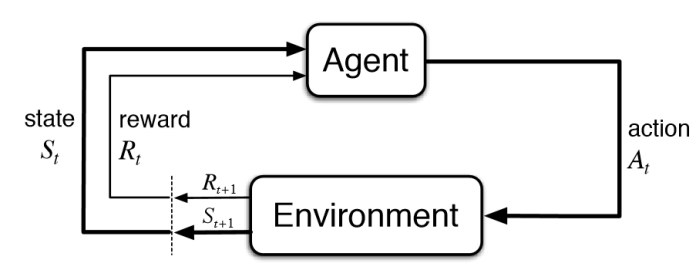
\includegraphics[width=0.8\linewidth]{rl.jpg}
	\caption{Illustration of Reinforcement Learning}
	\label{fig:statemachin}
\end{figure}

Implementing the above mentioned algorithms would be very time consuming, so we decided to use the Stable Baselines 3 library [TODO], which is a simlified version of OpenAI baselines. The SB3 library contains several implementations of state-of-the-art RL algorithms and useful tools to train, retrain and evaluate the models\cite{stablebase}.
[TODO: about the policy network]

\subsection{\normalsize{Environment}}

The environment gives us an 640x480 RGB image.
We have to preprocess this image, because feeding the original images to the CNN would be a waste of resources because it makes training process much slower, and the network can learn from smaller images just as well \cite{kalap}.

\subsubsection{\normalsize{Observations}}

Preprocessing actions are applied to the observations. These can be resizing the image, cropping the image, grayscale the image, segment the colors in it or stack the last n number of the frames.

\begin{figure}[H]
	\centering
	\begin{minipage}{.3\textwidth}
	\centering
	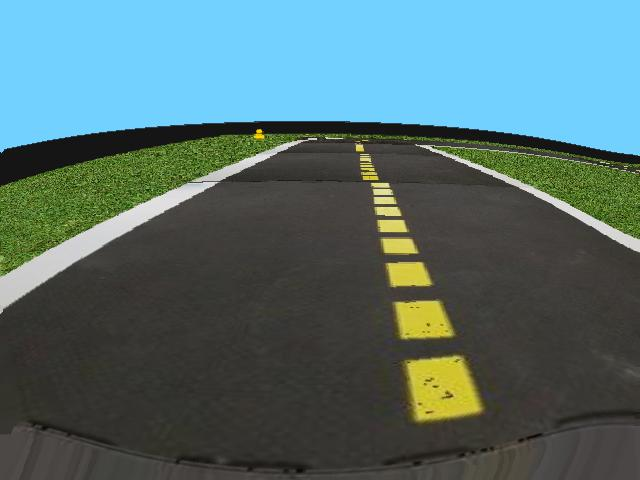
\includegraphics[width=0.8\linewidth]{rawobs.jpg}
	\caption{(a)}
	\end{minipage}%
	\begin{minipage}{.3\textwidth}
	\centering
	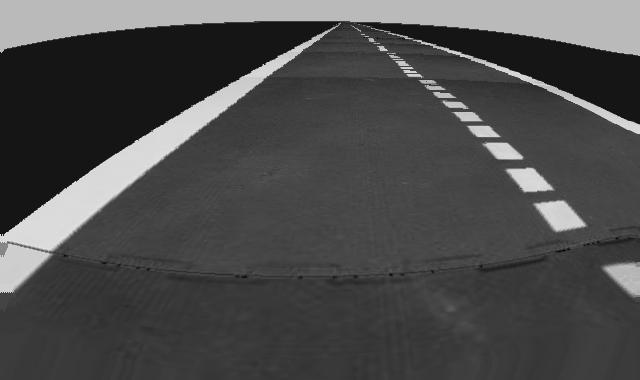
\includegraphics[width=0.8\linewidth]{grayscale.jpg}
	\caption{(b)}
	\end{minipage}%
\begin{minipage}{.3\textwidth}
	\centering
	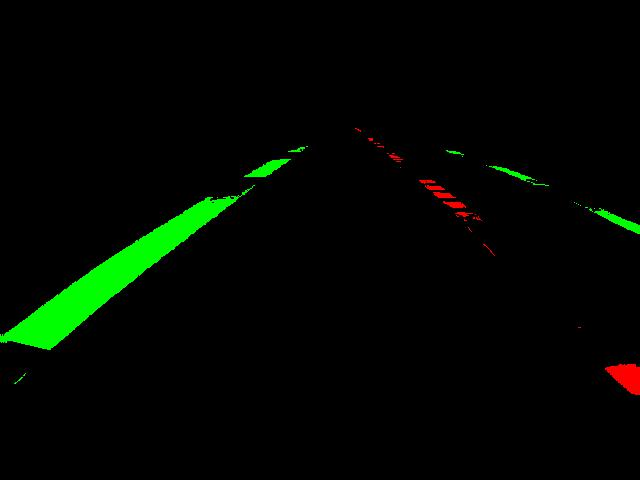
\includegraphics[width=0.8\linewidth]{colorseg.jpg}
	\caption{(c)}
\end{minipage}
\caption{Observations from the environment. (a) shows a raw observation, (b) shows a grayscaled image, (c) shows a color segmentated image}
\end{figure}

\subsubsection{\normalsize{Actions}}
\label{sec:actions}
Since the vehicle doesn't have turnable wheels, the turning must be achived by modifying the speed of the individual wheels. In the real life this speed is expressed as the PWM (Pulse Width Modulation) value of the applied voltage on the motor. For simplicity this value is normalized to 1 both in the simulation and the real life. For easier calculation the PWM value is not calculated dynamically it is statically coded at fix values which equates to three individual states. 
These states are forward, right turn, left turn.

\subsubsection{\normalsize{Rewards}}
\label{sec:rewards}
Just like any other engineering problem choosing optimal rewards are tricky and require lot of testing and empirical estimation. A poorly chosen reward function can be exploited by the agent. In our first test runs the agent got reward for staying on the path. The reward was increasing and we got long episodes which looked promising. After examining the data we discovered that the agent was rotating around in one place. 
It realized that the easiest way to maximize reward was not what we initially intended as a goal. To correct this we had to take in account the angle, position from the middle and speed of the agent.

\subsection{\normalsize{Evaluation}}
There are many ways to measure the performance of the trained agents, and for the sake of simplicity we chose two metrics for this purpose: survival time (in timesteps) and rewards received from the environment. Survival time tells us how many steps the agent took before either it went out of the road or the episode finished. A well-trained agent should stay on the road for the whole evaluation episode. 
Altough this provides valuable information, this metric does not tell much about performance on its own. Hence the rewards are also stored and evaluated to gain richer knowledge about the agents perfomance. The models were trained on the 'zigzag\_dists' map, because it offers a good balance between left and right turns and straight sections. In order to test how well the models learned to generalize, evaluation was done on three different maps: 'zigzag\_dists', 'loop\_empty', and 'udem1'.

\subsection{\normalsize{Hyperparameter Optimization}}
Reinforcement learning models are extremely sensitive to hyperparameter settings. A poor choice of hyperparameters can cause unstable performance or it could prevent convergence completely. Findig the right parameters for training can be a difficult job, and it is usually not a good idea to start tuning the parameters manually. Instead you can use an optimization library, that sets up sophisticated experiments to find the right hyperparameters for your usecase.

For our project we used the Optuna library, which offers several tools to dynamically explore the hyperparameter-space in a define-by-run style. The library features state-of-the-art alorithms for sampling and pruning, easy parallelization of experiments and visualization tools. In order to optimize our models, we used the Tree-structured Parzen Estimator (TPE) for sampling and the Median pruner for early termination of less promising trials. 
The studies were conducted with a budget of 100 trials and a maximum of 50000 steps, and evaluations at every 10000 steps. For optimizating the PPO model, we used an RTX 6000 workstation with 24GB VRAM and 46GB RAM, but for the A2C study, we had to use a GTX1060OC with 6GB of VRAM and 16GB RAM which was not enough to finish the study, so in that case the results are based on 47 finished trials. Tables \ref{tab:ppo} and \ref{tab:a2c} shows the optimized hyperparameters for the models.




\begin{table}[H]
	\begin{subtable}[h]{0.45\textwidth}
		\centering
		\begin{tabular}{|l | l|}
		\hline
		Learning rate schedule & constant  \\
		\hline
		Learning rate & 0.1324  \\
		\hline
		Norm. advantage & False  \\
		\hline
		n\_steps & 64  \\
		\hline
		Entropy coef. & 0.0015 \\
		\hline
		Use RMS prop. & False  \\
		\hline
		Gae. lambda & 0.98 \\
		\hline
		Max grad. norm. & 0.7  \\
		\hline
		vf coef. & 0.7373  \\
		\hline
		Activation  & tanh  \\
		\hline
		\end{tabular}
		\caption{A2C}
		\label{tab:a2c}
	\end{subtable}
	\hfill
	\begin{subtable}[h]{0.45\textwidth}
		\centering
		\begin{tabular}{|l | l |}
		\hline
		Learning rate schedule & linear \\
		\hline 
		Learning rate & 0.8764  \\
		\hline
		Batch size & 256  \\
		\hline
		n\_steps & 32  \\
		\hline
		Entropy coef. & 6.5699 \\
		\hline
		Clip range & 0.2  \\
		\hline
		Epochs & 5 \\
		\hline
		Gae. lambda & 0.92 \\
		\hline
		Max grad. norm. &  0.8 \\
		\hline
		vf coef. & 0.2425  \\
		\hline
		Activation & relu \\
		\hline
		\end{tabular}
		\caption{PPO}
		\label{tab:ppo}
	\end{subtable}
	\caption{Optimized model hyperparameters}
	\label{tab:hyp}
\end{table}




\section{\large{Results}}
The PPO and the A2C agents were trained in the gym-duckietown simulator, with concatenating the last 3, grayscaled observations, and using the 'steering' actions and the orientation rewards described in \autoref{sec:actions} and \autoref{sec:rewards}. The agents were trained on the 'zigzag\_dists' map for one million steps, using only 1 environment. Each episode lasted a maximum of 500 steps, because this proved to be enough to take at least a full round on the map for a reasonable agent. 
In order to examine the effects of the hyperparameter optimization, first we trained the models with mostly the default SB3 parameters, the only exception was the learning rate, which was set to a constant 0.0005 value. This was ment to be a baseline training to compare it with the optimized models. The main difference - besides the optimized parameters - was the use of 4 parallel environments and the 2 million steps long training. 
\autoref{t:zigzagdists}, \autoref{t:smalloop} and \autoref{t:udem1} shows the evaluation results on the different maps.


\begin{table}[H]
	\caption{Evaluation results on the 'zigzag\_dists' (seen) map}
	\begin{center}
	\begin{tabular}{|c| c| c| c| c|}
		\hline
	  & PPO (default) & A2C (default) & PPO (optimized) & A2C (optimized) \\
	\hline
	Mean episode reward & 11.51 & 74.24 & 128.19 & 74.24 \\
	\hline
	Mean episode length & 71.5 & 308.0 & 452.9& 308.0 \\
	\hline
	\end{tabular}
	\end{center}
	\label{t:zigzagdists}

	\caption{Evaluation results on the 'small\_loop' (unseen) map}
	\begin{center}
	\begin{tabular}{|c| c | c| c | c|}
		\hline
	  & PPO (default) & A2C (default) & PPO (optimized) & A2C (optimized) \\
	\hline
	Mean episode reward & 14.83 & 61.21 & 93.78 & 61.21 \\
	\hline
	Mean episode length & 69.8 & 219.5 & 311.6 & 219.5 \\
	\hline
	\end{tabular}
	\end{center}
	\label{t:smalloop}

	\caption{Evaluation results on the 'udem1' (unseen) map}
	\begin{center}
	\begin{tabular}{|c| c| c| c| c|}
		\hline
	  & PPO (default) & A2C (default) & PPO (optimized) & A2C (optimized) \\
	\hline
	Mean episode reward & 6.01 & 98.27 & 70.79 & 98.27 \\
	\hline
	Mean episode length & 38.2 & 359.6 & 262.7 & 359.6 \\
	\hline
	\end{tabular}
	\end{center}
	\label{t:udem1}
\end{table}

The evaluation results show us, that in the case of the PPO model, hyperparameter optimization significantly helped achieving higher rewards and longer runs, both in previously seen and unseen environments. 
But regarding the A2C model, the optimization seemingly did not help at all. It is unclear why this has occured, which means further examination of the training and evaluation conditions are needed for the A2C agent.
An other interesting result to consider, is the fact that the A2C model performed better on a map that it has never seen, which is also a more complex version of the 'small\_loop' map, with intersections and previously unseen objects like houses and ducks in the background.
Furthermore, the A2C model achieved much better results with its "default" hyperparameters than the PPO, which could mean it needs less optimization trials. 


\section{\large{Conclusion}}
In this work two reinforcement learning algorithms were trained to drive a two-wheel robot in a simulated environment. 
The models were compared with each other and their optimized versions using basic metrics from the simulation. 
It was found that optimization did help regarding the PPO model, but the A2C agent performed the same way. In order to understand the reasons behind this phenomena more in-depth experiments are needed. 
To further improve the results, longer optimization trials are necessary, with at least 100000 steps, and a variety of maps to train on, which can improve generalization and help avoid overfitting to a single map.
More evaluation methods could be used to elaborate further on the models performance, like transversal and angular deviations from the right lane centerline, or distance travelled in the ego lane.\\

(Disclaimer: This is not the final version of the document. Please see a more recent commit.)

\bibliography{bib}
%\addcontentsline{toc}{chapter}{Irodalomjegyzék}
%\bibliographystyle{plain}
\bibliographystyle{ieeetr}
%\bibliographystyle{unsrt}


\end{document}
